\documentclass[main.tex]{subfiles}
\begin{document}
\section{Shell}
\begin{figure}[H]
  \centering
  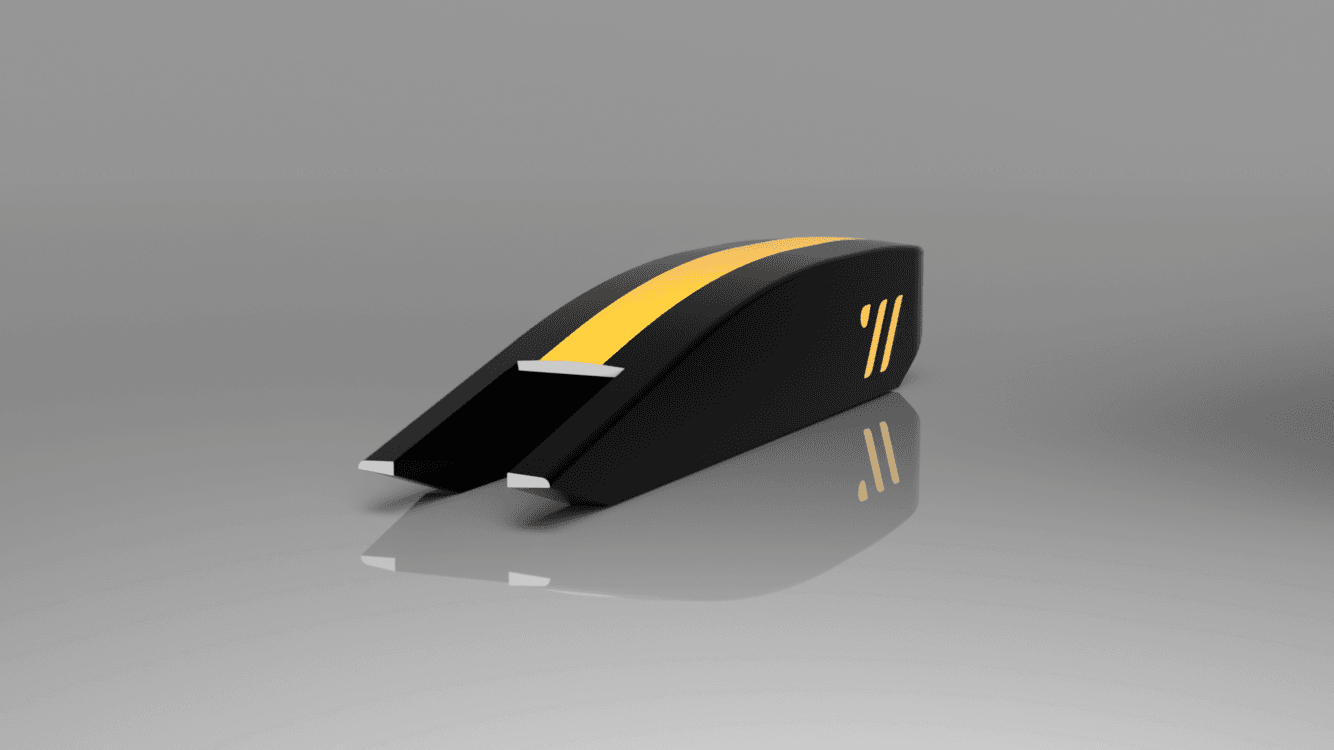
\includegraphics[width=0.75\textwidth]{images/BTTF_Render1.png}
  \caption{Proposed Goose III shell design}
  \label{fig:shell1}
\end{figure}

    \subsection{Overall Design}
    The Goose III shell will be constructed out of fibre glass with a foam core to increase rigidity. This shell will be directly mounted to the frame with rubber bushings in between in order to mitigate the effect of vibrations. A full breakdown of the shell properties is shown in \reftab{table:shelltable} \\
    
   	The cost breakdown of the Goose III shell includes all the equipment and physical material used in construction. As stated above, the shell will be constructed out of fibre glass layered to \SI{2.5}{mm} thickness along with a \SI{2.5}{mm} thick foam core to increase the rigidity of the shell. The fibre glass used in this construction will be plain woven hexcel style 7533 with a thickness of \SI{0.2}{mm}, as listed in the bill of materials for the shell (\reftab{table:shellmoney}). The fibreglass will be layered onto a male mold with a 50\% overlay per piece of $36"\times 50"$ fibreglass. The mold along with the fibre glass will be put through the vacuum infusion process where epoxy resin will fill up the area, bonding the fibre glass layers to the foam core. The shell will then be primed and painted before finally being mounted. 
    
\begin{table}
\centering
  \begin{tabular}{@{}ccc@{}} \toprule
    Parameter Type & Parameter & Value \\ \midrule
    \multirow{5}{4em}{Physical Properties} & Maximum Height [\si{mm}] & 500 \\
    & Maximum Width [\si{mm}] & 485 \\
    & Maximum Length [\si{mm}] & 2685 \\
    & Shell Thickness [\si{mm}] & 2.5 \\
    & Overall Mass [\si{kg}] & 11.96 \\
    \bottomrule
  \end{tabular}
  \caption{Shell specifications}
  \label{table:shelltable}
\end{table}

\subsection{Aerodynamics}    
Although the track is subject to a near-vacuum pressure, the remaining air will still have an effect on the overall drag experienced by the pod. In order to calculate this value and design around it, a CFD analysis was performed in ANSYS 18.0. A new shell was designed and compared to the shell used in the previous competition. An overview of the simulations is shown in \reftab{table:aerotable}.
\begin{table}
\centering
\begin{tabulary}{\linewidth}{@{}Lrll@{}}
\toprule
Parameter Type & Parameter & Goose II Shell & Goose III Shell \\
\midrule
\multirow{3}{4em}{Meshing Parameters} & Maximum Face Size [\si{m}] & 0.08 & 0.08 \\
& Number of Nodes & 96248 & 100404 \\
& Number of Elements & 510094 & 507358 \\
\midrule
\multirow{2}{4em}{Fluid Parameters} & Fluid & Air at \SI{25}{\celsius} & Air at \SI{25}{\celsius} \\ 
& Pressure [\si{Pa}] & 815 & 815 \\
\midrule
\multirow{3}{4em}{Boundary Conditions} & Inlet & Normal Velocity of \SI{100}{m/s} & Normal Velocity of \SI{100}{m/s} \\
& Outlet & Average Static Pressure of 0 Pa & Average Static Pressure of 0 Pa \\
& Walls & No-Slip Condition & No-Slip Condition \\
\midrule
\multirow{4}{4em}{Solver Parameters} & Turbulence Model & k-$\epsilon$ & k-$\epsilon$ \\ 
& Wall Function & Scalable & Scalable \\ 
& Advection Scheme & High Resolution & High Resolution \\ 
& Convergence Criteria & RMS $\leq 10^{-4}$ & RMS $\leq 10^{-4}$ \\ 
\bottomrule
\end{tabulary}
\caption{CFD simulation parameters}
\label{table:aerotable}
\end{table}
Each pod was placed one meter from the inlet in a 9m long tube fit to the SpaceX track specifications. The mesh acquired for the two simulations is shown in \reffig{fig:cfdmesh}.
\begin{figure}
\centering
\begin{subfigure}[h]{0.72\textwidth}
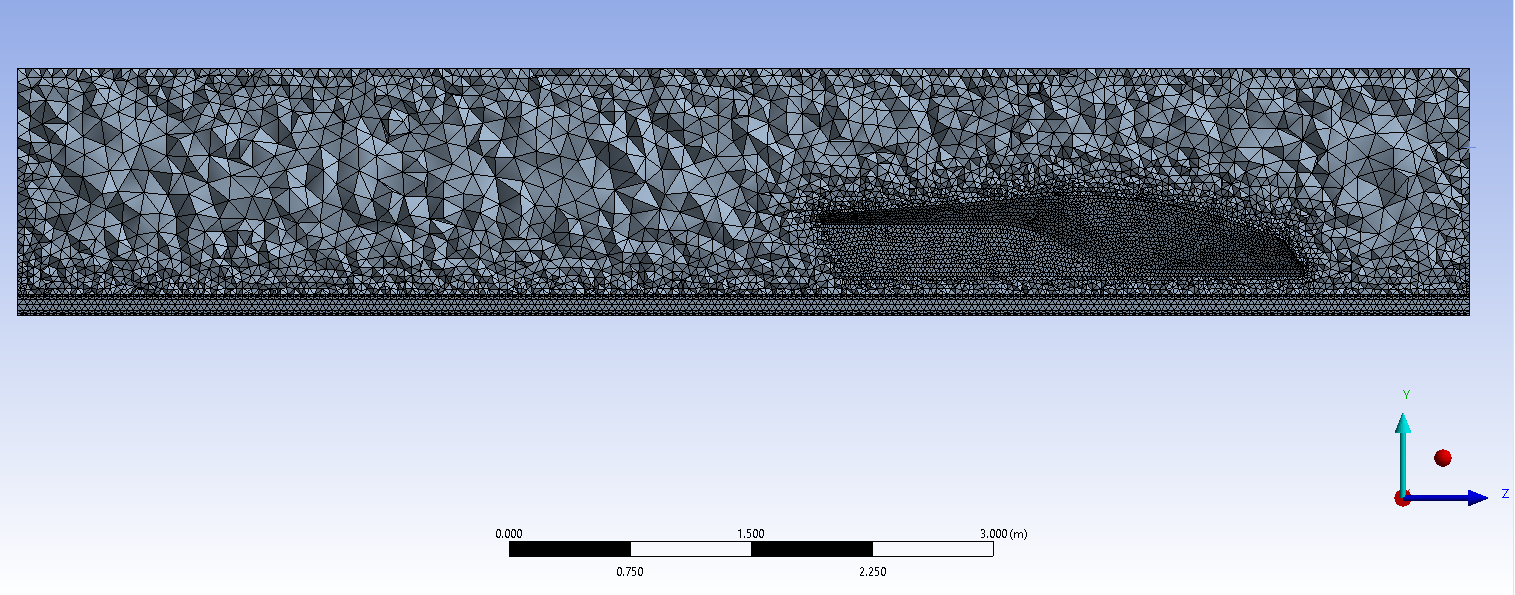
\includegraphics[width=\textwidth]{images/Goose_2_Mesh.PNG}
\caption{Goose II shell mesh}
\end{subfigure}
\begin{subfigure}[h]{0.72\textwidth}
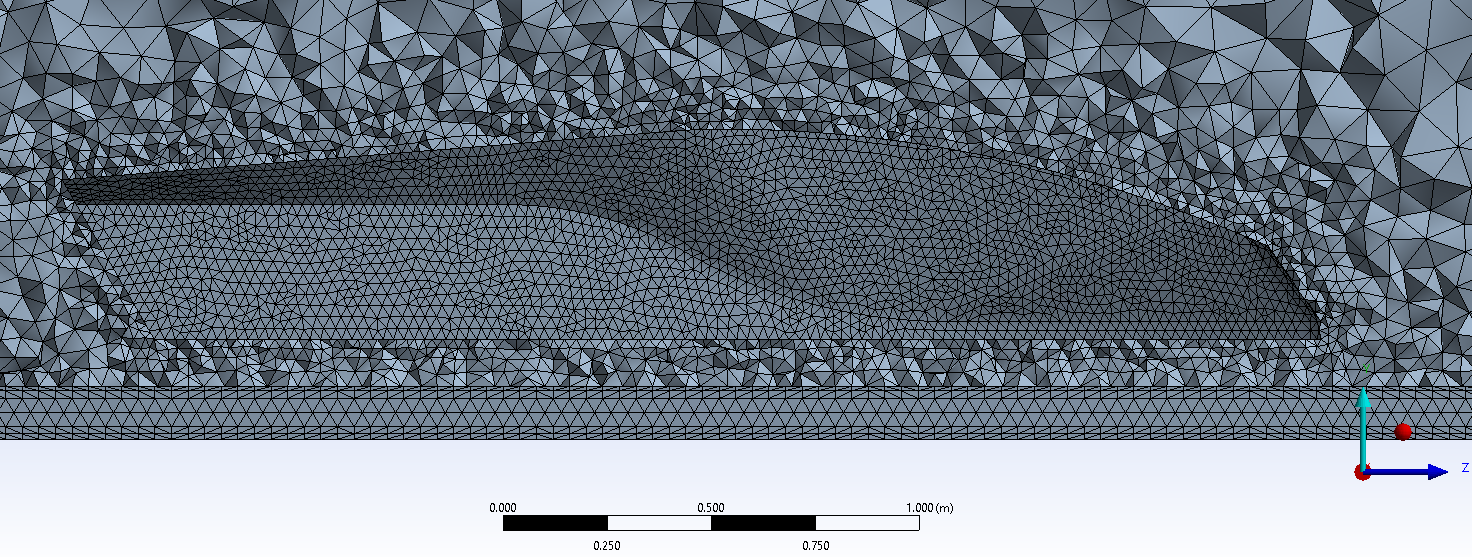
\includegraphics[width=\textwidth]{images/Goose_2_Mesh2.PNG}
\caption{Zoomed in Goose II shell mesh}
\end{subfigure}
\begin{subfigure}[h]{0.72\textwidth}
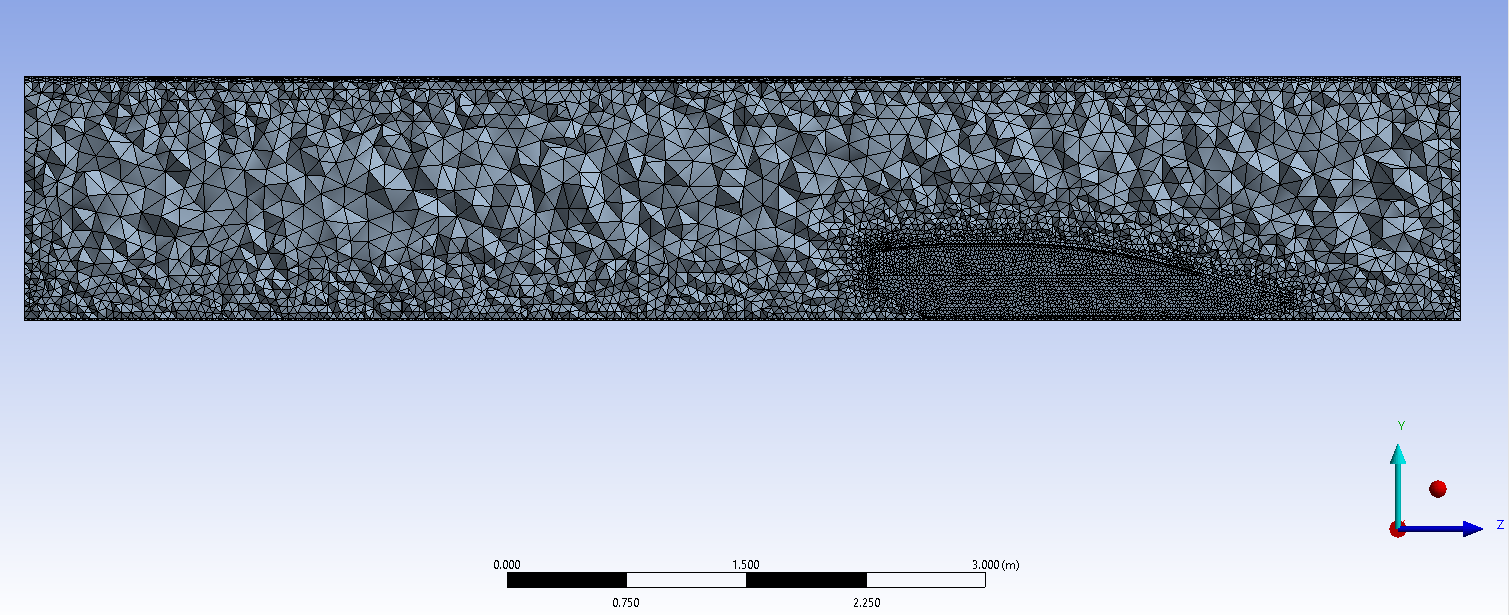
\includegraphics[width=\textwidth]{images/Victor_Mesh.PNG}
\caption{Proposed Goose III shell mesh}
\end{subfigure}
\begin{subfigure}[h]{0.72\textwidth}
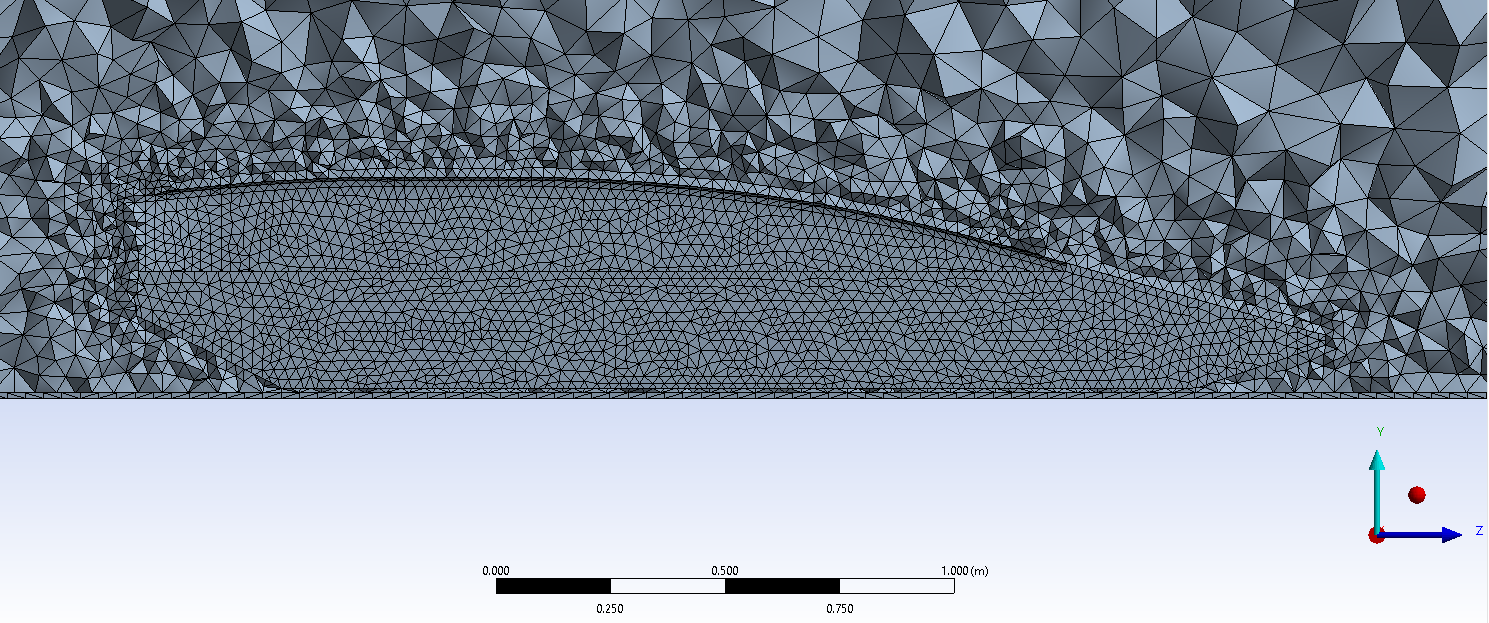
\includegraphics[width=\textwidth]{images/Victor_Mesh2.PNG}
\caption{Zoomed in proposed Goose III shell mesh}
\end{subfigure}
\caption{Mesh used for CFD simulations.}
\label{fig:cfdmesh}
\end{figure}
Running these simulations, the results in the form of pressure contours on the pod are shown in \reffig{fig:pressurecontours}.
\begin{figure}
\centering
\begin{subfigure}[h]{0.75\textwidth}
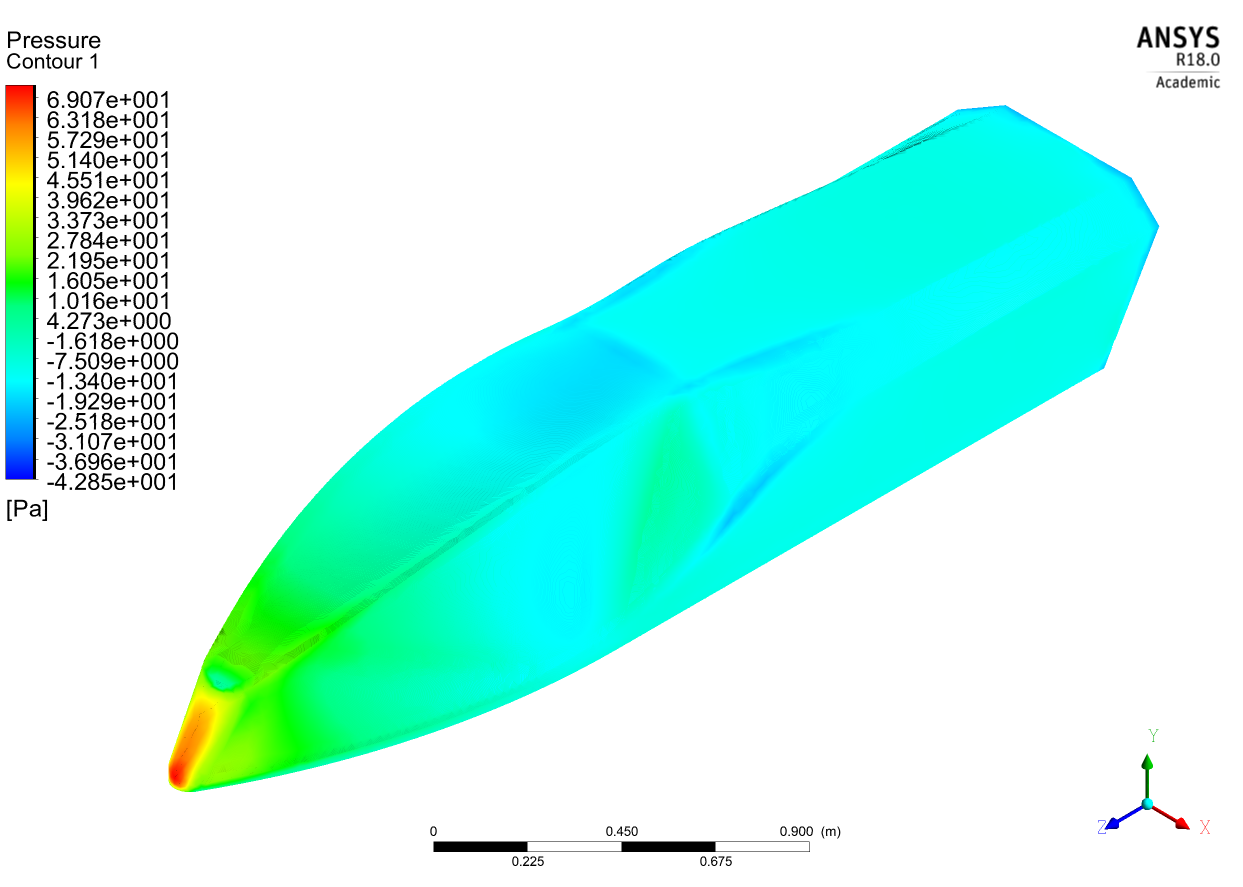
\includegraphics[width=\textwidth]{images/Test_3_Pressure_Contour.png}[h!]
\caption{Goose II pressure contours.}
\end{subfigure}
\begin{subfigure}[h]{0.75\textwidth}
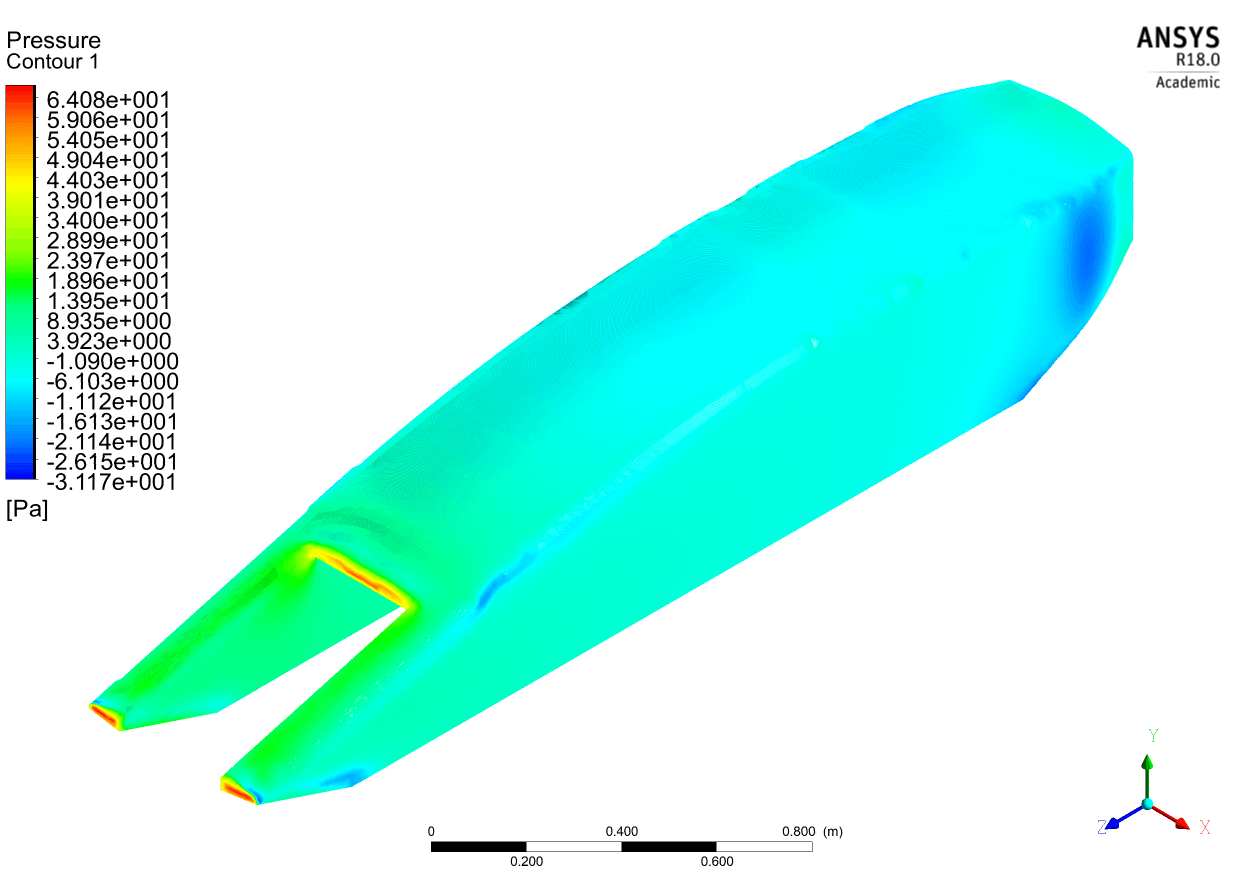
\includegraphics[width=\textwidth]{images/Test_4_Pressure_Contour.png}[h!]
\caption{Proposed Goose III pressure contours.}
\end{subfigure}
\caption{Pressure contours on the body of the two different pods.}
\label{fig:pressurecontours}
\end{figure}
\reffig{fig:pressurecontours} shows how little stress the pod body is under due to aerodynamic effects. This is summarized by the total drag forces experienced by the pod in each simulation shown in \reftab{table:aerotable2}
\begin{table}[h!]
\centering
\begin{tabular}{c c c} 
\hline
Parameter & Goose II Shell & Goose III Shell \\
\hline
Total Aerodynamic Drag [N] & 9.47 & 4.37\\
Drag Coefficient & 1.06 & 0.58\\
\hline
\end{tabular}
\caption{CFD simulation results.}
\label{table:aerotable2}
\end{table}
As shown in \reftab{table:aerotable2}, due to the near-vacuum pressure in the tube, the drag experienced from the pod is very low. The calculated drag coefficient is 0.58 with a drag force of 4.37N for the proposed shell. To prove the insignificance of this value, it is approximately equal to the weight exerted by 3.84 bananas. The overall drag will have a negligible effect on the performance so no further aerodynamic analysis was performed.

In terms of the Kantrowitz limit, this can be calculated with the following equation:
\begin{equation}
\frac{A_{\textrm{bypass}}}{A_{\textrm{tube}}}=\bigg[\frac{\gamma - 1}{\gamma + 1}\bigg]^{\frac{1}{2}}\bigg[\frac{2\gamma}{\gamma + 1}\bigg]^{\frac{1}{\gamma - 1}}\bigg[1 + \frac{2}{\gamma - 1}\frac{1}{M^{2}}\bigg]^{\frac{1}{2}}\bigg[1 - \frac{\gamma - 1}{2\gamma}\frac{1}{M^{2}}\bigg]^{\frac{1}{\gamma - 1}}
\end{equation}
When calculating the ratio of the tube area to the bypass area around the pod with $\gamma= 1.400$ and Mach 0.3, it was found the the equation is not valid. This is due to the fact that the equation is only valid for supersonic or near-supersonic velocities. More specifically, the equation is valid for Mach 0.378 or greater. Thus, it can be concluded that the Kantrowitz limit does not apply to our pod design and choked flow will not occur since the mach number experienced by our pod is only roughly 0.30.\\

    \subsection{Structural}
To increase the stability and decrease the loading on the shell, the shell will be constructed with a foam core. This will then be mounted to the frame with rubber bushings added to mitigate any propagating vibrations. The shell will be constructed out of fibreglass due to the high strength and lightweight characteristics. The forces on the shell will then be due to the inertia of the shell, as well as aerodynamic forces from the remaining air in the tube. With the weight of the shell being roughly \SI{12}{kg}, maximum acceleration being about \SI{9}{m/s^2}, and the total aerodynamic drag of \SI{4}{N}, the total force on the shell is about \SI{120}{N}. It is reasonable to assume that the force will not cause any damage on the shell due to the materials chosen. 

\end{document}
